\icode{N24Z-MI-SI-L3-261109-002}
\nceeID[3]{2024浙江1月}{6}
如图所示，在同一竖直平面内，小球\(A\)、\(B\)上系有不可伸长的细线\(a\)、\(b\)、\(c\)和\(d\)，其中\(a\)	的上端悬挂于竖直固定的	支架上，\(d\)跨过左侧定滑轮、\(c\)跨过右侧定滑轮分别与相同配重\(P\)、\(Q\)相连，调节左、右两侧定滑轮高度达到平衡。已知小球\(A\)、\(B\)和配重\(P\)、\(Q\)的质量均为\qty{50}{g}，细线\(c\)、\(d\)平行且与水平成\(\theta =\)\,\qty{30}{\degree}（不计摩擦），则细线\(a\)、\(b\)的拉力分别为\paren[]

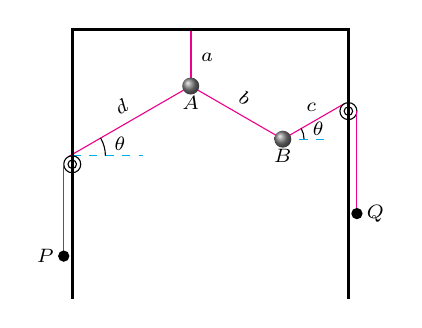
\begin{tikzpicture}[scale=.9,font=\scriptsize]
	\coordinate (A) at({1.25*sqrt(3)+.06},{-.25-.06*sqrt(3)});
	\coordinate (A1) at({1.25*sqrt(3)+.18},{-.25-.06*sqrt(3)});
	\coordinate (B) at({-sqrt(3)+.06},{-1-.06*sqrt(3)});
	\coordinate (B1) at({-sqrt(3)-.06},{-1-.06*sqrt(3)});
	\draw[magenta] (0,0)--node[above,black,rotate=-30]{\(b\)}(-30:1.5)--++(30:1) (0,0)--node[above,black,rotate=30]{\(d\)}(-150:2);
	\draw[thick,magenta] (0,0)--node[right,black]{\(a\)}(0,.8);
	\draw[dashed,cyan] (-30:1.5)--(-30:1.5-|2,0) ({-sqrt(3)+.06},{-1-.06*sqrt(3)+.12})--++(0:1);
	\draw ({0.75*sqrt(3)+.3},-.75) arc(0:30:.3) ({-sqrt(3)+.56-.12*tan(15)},{-1-.06*sqrt(3)+.12}) arc(0:30:.5);
	\shade[ball color=gray] (-30:1.5) circle(.12);
	\shade[ball color=gray] (0,0) circle(.12);
	\draw[thin] (A) circle(.12) (A) circle(.06);
	\draw[magenta] (A1)--(A1|-0,-1.8);
	\draw[thin] (B) circle(.12) (B) circle(.06);
	\draw[magenta] (B1)--(B1|-0,-2.4);
	\draw[very thick] (B|-0,-3)--(B|-0,.8)--(A|-0,.8)--(A|-0,-3);
	\fill (B1|-0,-2.4)node[left]{\(P\)} circle(.08);
	\fill (A1|-0,-1.8)node[right]{\(Q\)} circle(.08);
	\node at(0,0)[below]{\(A\)};
	\node at(-30:1.5)[below]{\(B\)};
	\node at(-1,-.82){\(\theta\)};
	\node at(1.8,-.6){\(\theta\)};
	\node at(1.7,-.3){\(c\)};
\end{tikzpicture}
\begin{choices}
	\item \qty{2}{N}\quad\qty{1}{N}
	\item \qty{2}{N}\quad\qty{0.5}{N}
	\item \qty{1}{N}\quad\qty{1}{N}
	\item \qty{1}{N}\quad\qty{0.5}{N}
\end{choices}
\begin{answer}
	D\qquad 提示：分解力，合成力。
\end{answer}